%------------------------------------------------------------------------
\begin{frame}
\frametitle{Radial Basis Function Expansion\\
\csub{\small Not an orthogonal basis}}

\begin{equation*}
f(x) = \sum_{n=0}^{N-1} c_n e^{-(x-x_i)^2/\Delta^2}  
\end{equation*}
\begin{center}
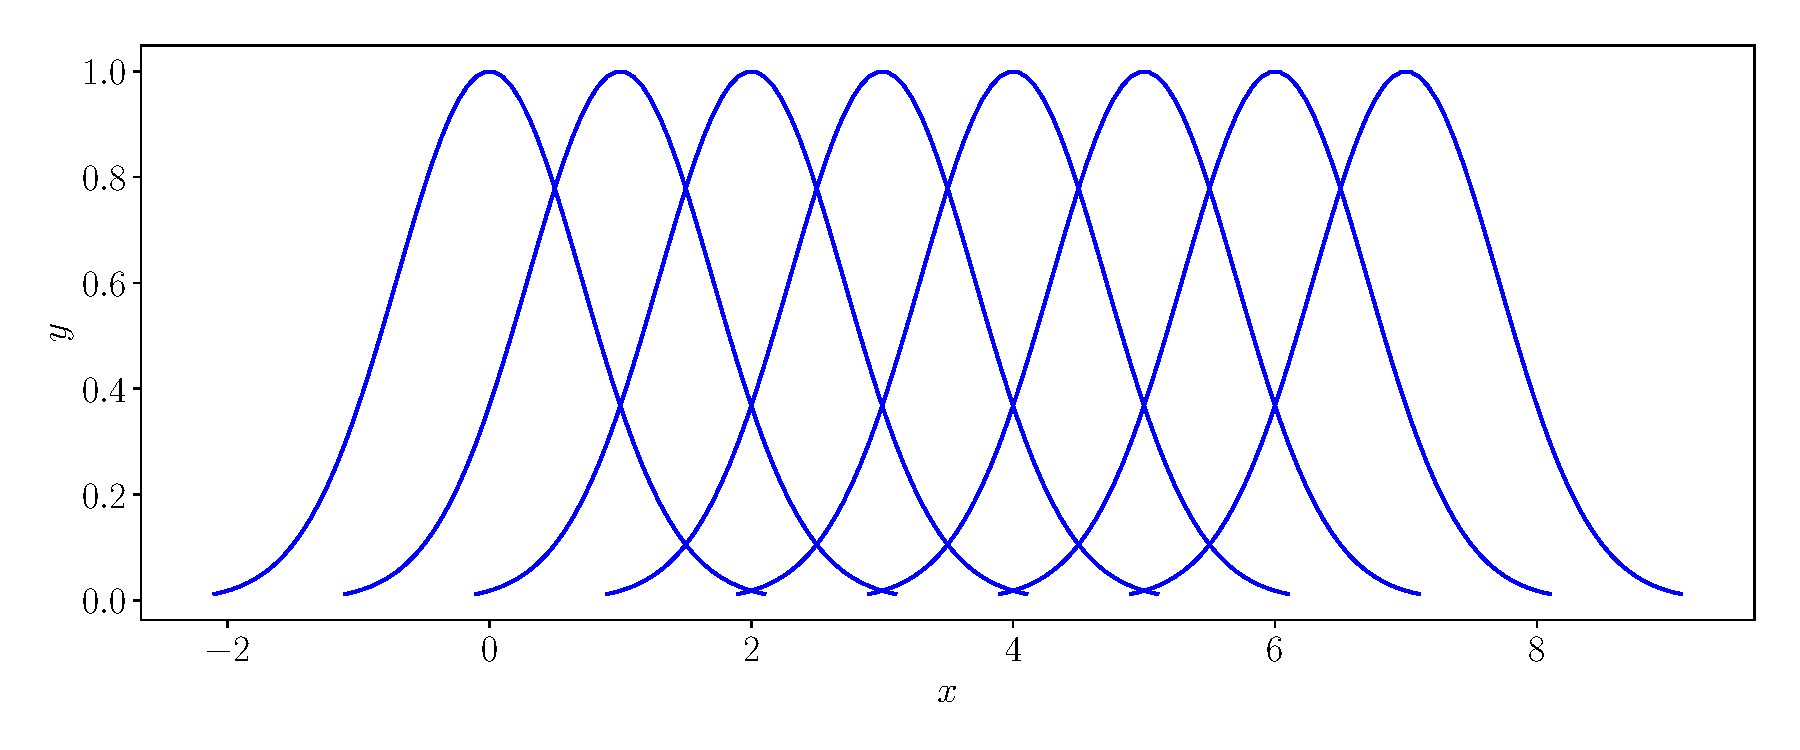
\includegraphics[width=5.5in]{rbf.pdf}
\end{center}
\end{frame}
%------------------------------------------------------------------------
%------------------------------------------------------------------------
\begin{frame}
\frametitle{RBF Cookbook\\
\textcolor{egg}{\large Wide spectrum of applications in applied math}}
Here, $r = |\mathbf{x}|$ is length in $n$ dimensions, such that $\mathbf{x} \in {\cal R}^n$ 
\begin{align*}
 \hilite{Gaussian (GRBF)}~~~\phi(r) &~= e^{-(\varepsilon r)^2} \\
 \sgreen{Multiquadric}~~~\phi(r) &~= \sqrt{1+(\varepsilon r)^2}  \\
 \sgreen{Inverse Multiquadric}~~~\phi(r) &~= \frac{1}{\sqrt{1+(\varepsilon r)^2}} \\
 \sgreen{Inverse Quadratic}~~~\phi(r) &~= \frac{1}{1+(\varepsilon r)^2} \\
 \sgreen{Polyharmonic Spline}~~~\phi(r) &~= r, \, r^3, \, r^5, \ldots \\
 \sgreen{Thin-Plate Spline}~~~\phi(r) &~= r^2 \ln(r) \\
\end{align*}
\end{frame}
%------------------------------------------------------------------------

%------------------------------------------------------------------------
\begin{frame}
\frametitle{RBF Interpolation {\large[Fornberg, SIAM J.~Sci.~Comput.~33 (2011)]}\\
\textcolor{egg}{\large Mesh-free approximation in $n$-dimensions}}

\begin{enumerate}
\item<1-> Pick a radial basis function $\phi(r)$
\item<2-> Collect some scattered data $\{\xvec_k,f_k\}$ for $k=1,2,\ldots,N$.
\item<3-> Make an RBF interpolant
  \begin{equation*}
    s(\xvec,\varepsilon) = \sum_{k=1}^N \lambda_k \phi(|\xvec-\xvec_k|)
  \end{equation*}
\item<4-> Compute the coefficients $\lambda_k$ as the solution of the linear system
  \begin{equation*}
    A_{jk} \lambda_k = f_j \quad\mbox{where}\quad A_{jk} = \phi(|\xvec_j-\xvec_k|)
  \end{equation*}
\item<5-> As $\varepsilon \rightarrow 0$ accuracy increases but $A_{jk}$ becomes \alert{ill-conditioned}
\end{enumerate}

\end{frame}
%------------------------------------------------------------------------
\newcommand\cwid{14cm}
%------------------------------------------------------------------------
\begin{frame}
\frametitle{GRBF Illustration\\
\textcolor{egg}{\large $N=4$}}
\begin{center}
  \vspace{-3mm}
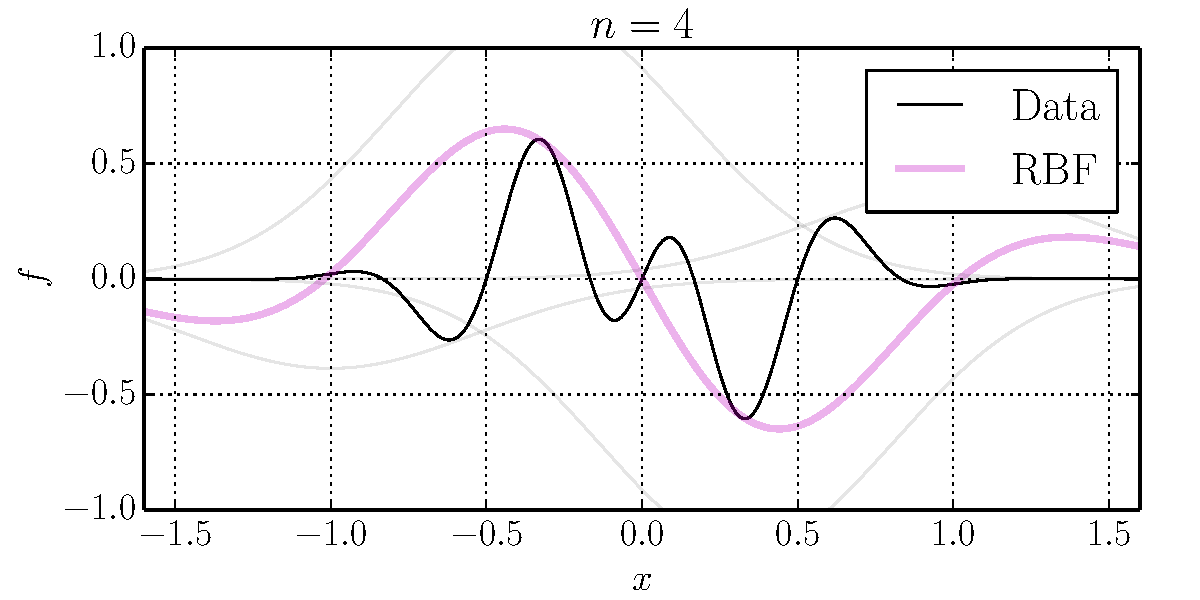
\includegraphics[width=\cwid]{4n.pdf}
\end{center}
\end{frame}
%------------------------------------------------------------------------
%------------------------------------------------------------------------
\begin{frame}
\frametitle{GRBF Illustration\\
\textcolor{egg}{\large $N=6$}}
\vskip -5mm
\begin{center}
  \vspace{-3mm}
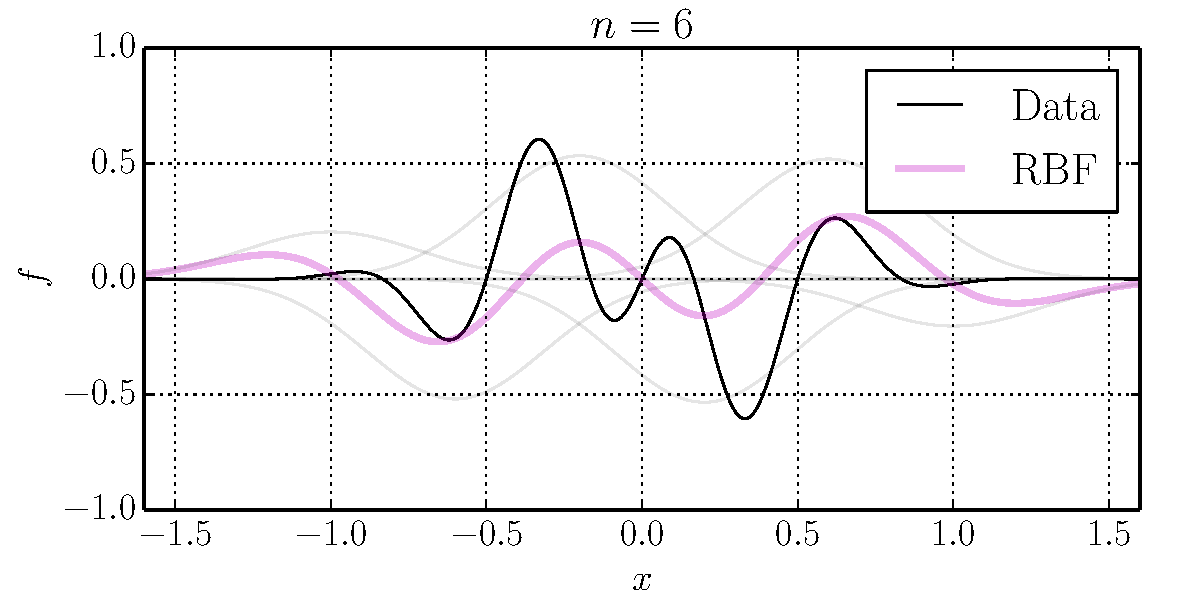
\includegraphics[width=\cwid]{6n.pdf}
\end{center}
\end{frame}
%------------------------------------------------------------------------
%------------------------------------------------------------------------
\begin{frame}
\frametitle{GRBF Illustration\\
\textcolor{egg}{\large $N=8$}}
\begin{center}
  \vspace{-3mm}
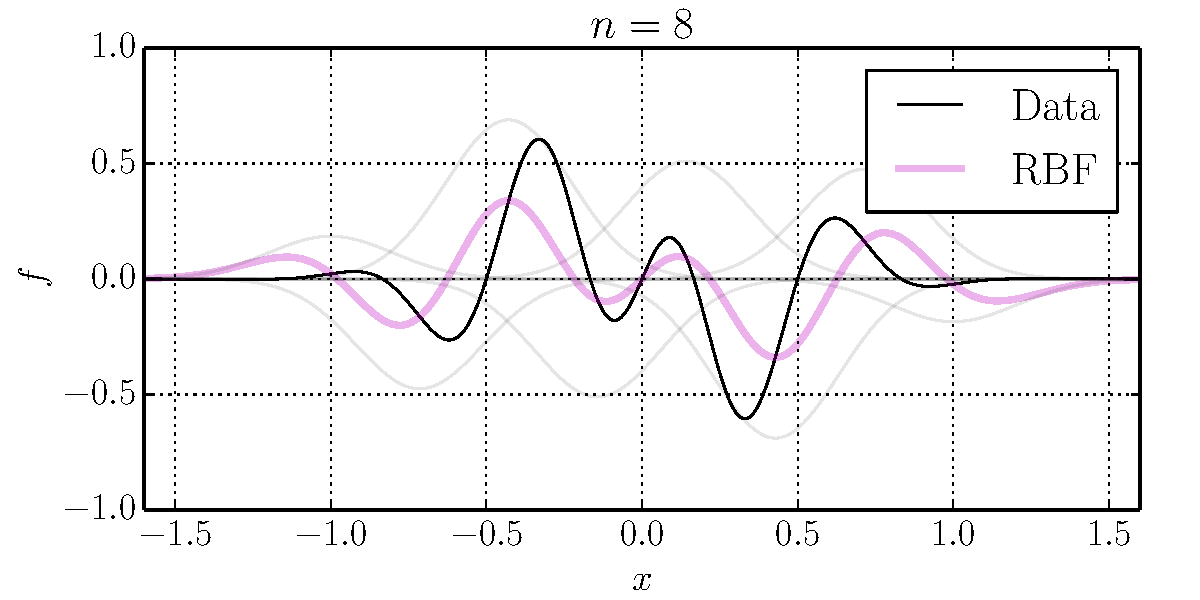
\includegraphics[width=\cwid]{8n.pdf}
\end{center}
\end{frame}
%------------------------------------------------------------------------
%------------------------------------------------------------------------
\begin{frame}
\frametitle{GRBF Illustration\\
\textcolor{egg}{\large $N=10$}}
\begin{center}
  \vspace{-3mm}
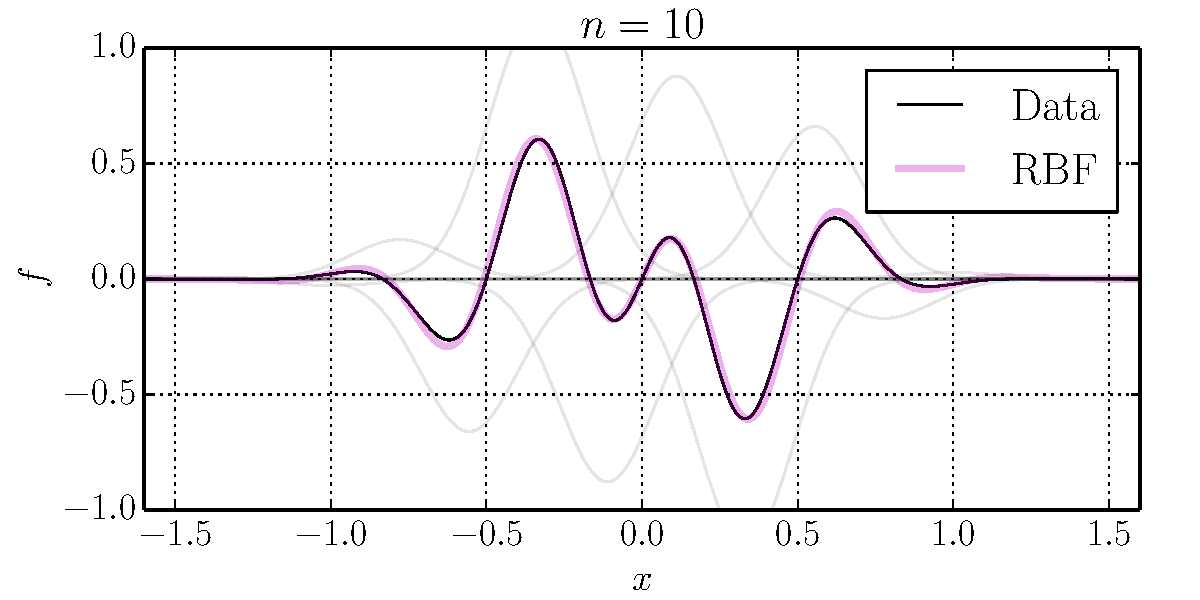
\includegraphics[width=\cwid]{10n.pdf}
\end{center}
\end{frame}
%------------------------------------------------------------------------

%------------------------------------------------------------------------
\begin{frame}
\frametitle{6D Fokker-Planck-Landau Equation\\
\textcolor{egg}{\large Everything: MHD, gyrokinetics, cyclotron waves, you name it.}}

\begin{equation*}
  \frac{\partial f_a}{\partial t} + \vvec\cdot\nabla f_a
  + \frac{e_a}{m_a} \left( \evec + \frac{\vvec}{c} \times \bvec \right) \cdot
  \frac{\partial f_a}{\partial \vvec}
  = \onslide<2->{\textcolor{blue}{\sum_b C_{ab}(f_a,f_b) + S_a}} 
\end{equation*}

\begin{align*}
  \onslide<1->{f_a(\xvec,\vvec,t) &~\longrightarrow \mbox{6D distribution function for species $a$}} \\
  \onslide<2->{\textcolor{blue}{C_{ab}} &~\longrightarrow \textcolor{blue}{\mbox{Nonlinear (bilinear) Collision Operator}}}
\end{align*}

\begin{center}
  \onslide<3->{This is a \hilite{complex integro-differential} equation in $\vvec$}
\end{center}

\end{frame}
%------------------------------------------------------------------------

%------------------------------------------------------------------------
\begin{frame}
\frametitle{Nonlinear Coulomb Collision Operator\\
\textcolor{egg}{\large Numerical treatment extremely challenging}}
\vskip -2mm
Collision operator
\vskip -2mm
\begin{equation*}
C_{ab}(f_a,f_b) = \frac{\partial}{\partial\vvec}\cdot\left[\mathbf{A}_{ab}\,f_a
+ \frac{\partial}{\partial\vvec}\cdot\left(\mathbb{D}_{ab}\,f_a\right)\right]
\end{equation*}
Friction and diffusion coefficients
\begin{align*}
\mathbf{A}_{ab}=\;L^{ab}\left(1+\frac{m_a}{m_b}\right)\frac{\partial\varphi_b}{\partial\mathbf{v}}
\qquad  \mathbb{D}_{ab}=-L^{ab}\frac{\partial^2\psi_b}{\partial\mathbf{v}\partial\mathbf{v}}
\end{align*}
\vskip -2mm
Rosenbluth potentials
\hbox{
\begin{minipage}{0.2\textwidth}
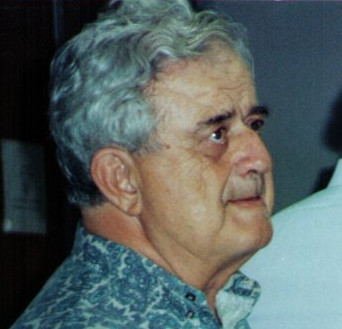
\includegraphics[width=1.1\linewidth,keepaspectratio=true]{mnr.jpg}
\end{minipage}
\begin{minipage}{0.7\textwidth}
\vskip -3mm
  \begin{align*}
\varphi_b(\mathbf{v},t)=&-\frac{1}{4\pi}\int \dvp \, f_b(\vvecp,t)\frac{1}{|\vvec-\vvecp|} \\
\psi_b(\mathbf{v},t)=&-\frac{1}{8\pi}\int \dvp \, f_b(\vvecp,t)|\vvec-\vvecp|
\end{align*}
\end{minipage}
}
\end{frame}
%------------------------------------------------------------------------
%------------------------------------------------------------------------
\begin{frame}
\frametitle{Plasma Equilibrium\\
\textcolor{egg}{\large The Shifted Maxwellian}}

\begin{center}
  \hilite{Connection with plasmas and systems close to equilibrium}
\end{center}

\begin{itemize}
\item<1->The distribution of particles in the DIII-D core is nearly
  \begin{equation*}
    f_a = \frac{n_a}{(\pi/\gamma_a)^{3/2}} e^{-\gamma_a (\vvec-\mathbf{V})^2}
    \;\;\; \mbox{where} \;\;\;  \gamma_a \doteq \frac{m_a}{2 T_a}
  \end{equation*}
\item<2->The error is typically less than $1\%$ (gyrokinetic ordering)
\item<3->This is a \hilite{Gaussian RBF} with center $\mathbf{V}$ and width $\gamma_a$
\item<4->GRBFs are a \hilite{natural basis} for plasma simulation
\item<5->\hilite{Magic} property:  $C_{aa}(f_a,f_a) = 0$
\end{itemize}
\end{frame}
%------------------------------------------------------------------------
%------------------------------------------------------------------------
\begin{frame}
\frametitle{GRBFs $=$ Shifted Maxwellians\\
\textcolor{egg}{\large Universal functions in statistical mechanics}}

\hilite{Basic strategy:}~~Expand $f_a$ in series of shifted Maxwellians

\begin{equation*}
f_a(\xvec,\vvec,t) = \sum_i \bwi(\xvec,t) \,
\left(\frac{\gamma_i}{\pi}\right)^{3/2}
e^{-\gamma_i(\vvec-\vvec_i)^2}
\end{equation*}

\hilite{Fluid moments:} simple, elegant weighted sums:

\begin{equation*}
n_a = \sum_i \bwi (\xvec,t)
\quad\mbox{and}\quad
n_a \mathbf{V}_a = \sum_i \bwi (\xvec,t) \, \vvec_i(\xvec)
\end{equation*}

\hilite{Free parameters:} widths (bases) and centers (mesh):
\begin{equation*}
  \{ \gamma_i, \vvec_i \} \quad\mbox{... or alternatively} \; \gamma_i = \frac{m_a}{2\trbf_i^a}
\end{equation*}

\end{frame}
%------------------------------------------------------------------------

%------------------------------------------------------------------------
\begin{frame}
\frametitle{Can Evaluate Rosenbluth Potentials Analytically\\
\textcolor{egg}{\large Result is exact in the space of GRBFs}}

Rosenbluth potentials are evaluated \hilite{exactly}:
%
\begin{align*}
f_a(\vvec) &~=
\sum_i \bwi \left(\frac{\gamma_i}{\pi}\right)^{3/2} e^{-y^2} \\
-4 \pi \, \varphi_a(\vvec) = \int \dvp \, f_b(\vvecp,t)\frac{1}{|\vvec-\vvecp|} &~=
\sum_i \bwi \left(\gamma_i\right)^{1/2} \frac{\mathrm{Erf}(y)}{y}
\\
-8 \pi \, \psi(\vvec) = \int \dvp \, f_b(\vvecp,t){|\vvec-\vvecp|} &~=
\sum_i \bwi \left( \gamma_i \right)^{-1/2}
\left[ \left(y+\frac{1}{2y}\right) \mathrm{Erf}(y)
+ \frac{1}{\sqrt{\pi}} \, e^{-y^2} \right]
\\
\end{align*}
%
where $y = \sqrt{\gamma_i} | \vvec - \vvec_i|$.
\end{frame}
%------------------------------------------------------------------------

%------------------------------------------------------------------------
\begin{frame}
\frametitle{Collision operator also has analytic form\\
\textcolor{egg}{\large Result is exact in the space of GRBFs}}

The full collision operator is simply a sum of products of weights
\begin{equation*}
C_{ab}(f_a,f_b) = \sum_i \sum_k \textcolor{blue}{w^a_i} \, \textcolor{blue}{w^b_k} \, C^{ab}_{ik}(\vvec)
\end{equation*}
%
where
%
\begin{align*}
C^{ab}_{kl}(\mathbf{v})=L^{ab}\left[\frac{m_a}{m_b}f_i^a f_k^a+
 \left(\frac{m_a}{m_b}-1\right)\frac{\partial\varphi_i^a}{\partial\vvec}\cdot\frac{\partial f_k^b}{\partial\vvec}
-\frac{\partial^2\psi_i^a}{\partial\vvec\partial\vvec}:\frac{\partial^2f_k^b}{\partial\vvec\partial\vvec}\right].
\end{align*}

\end{frame}
%------------------------------------------------------------------------

%------------------------------------------------------------------------
\begin{frame}
\frametitle{Nonlinear GRBF equations \\
\textcolor{egg}{\large Fluid-like equations with no velocity dependence}}
%
\vspace{2mm}
\begin{tcolorbox}[%
colback=blue!3,
colframe=blue!40!black,
title={Fluid equations for $w_1^a, \, w_2^2, \, \ldots, \, w_N^a$}]
\begin{equation*}
\begin{split}
\sum_{i=1}^N M_{ij} \left\{
\frac{\partial\bwi}{\partial t} + \vvec_j\cdot\nabla \bwi +
\frac{e_a}{\trbf_i^a} \left[
(\vvec_i-\vvec_j) \cdot \evec + \frac{1}{c} (\vvec_i \times \vvec_j) \cdot \bvec \right] \bwi
\right\} \\
= \sum_{i,k,b} C_{ik,j}^{ab} \, \textcolor{blue}{w_i^a} \, \textcolor{blue}{w_k^b}
\end{split}
\end{equation*}
\end{tcolorbox}
\vspace{-2mm}
\begin{align*}
\mbox{Projection weights:}  \quad & M_{ij} = \left(\frac{\gamma_j}{\pi}\right)^{3/2}
e^{-\gamma_j\left(\mathbf{v}_i-\mathbf{v}_j\right)^2} \; , \;\; \trbf_i^a = \frac{m_a}{2\gamma_i}\\
\mbox{Centers:} \quad & \vvec_1(\xvec), \, \vvec_2(\xvec), \, \ldots, \, \vvec_N(\xvec) \\
\mbox{Widths:} \quad & \gamma_1(\xvec), \, \gamma_2(\xvec), \, \ldots, \, \gamma_N(\xvec)
\end{align*}

\end{frame}
%------------------------------------------------------------------------

%------------------------------------------------------------------------
\begin{frame}
\frametitle{Fluid Moments\\
\textcolor{egg}{\large Exact in the space of GRBFs}}

\begin{align*}
\sgreen{Density}~~~n_a &~= \sum_i \bwi \\
\sgreen{Velocity}~~~n_a \mathbf{V}_a &~= \sum_i \bwi \, \vvec_i(\xvec) \\
\sgreen{Temperature}~~~\frac{3}{2} n_a T_a &~= \sum_i \bwi
\left[ \frac{3}{2} \trbf_i^a + \frac{1}{2} m_a (\vvec_i-\mathbf{V}_a)^2 \right] \\
\sgreen{Momentum flux}~~~\left( \Pi_a \right)_{\mu\nu} &~= \sum_i \bwi \, m_a
\Big[ \trbf_i^a + (\vvec_i)_\mu (\vvec_i)_\nu  \Big] \\
\sgreen{Energy flux}~~~\mathbf{Q}_a &~= \sum_i \bwi \, \vvec_i
\left[ \frac{5}{2} \trbf_i^a + \frac{1}{2} m_a v_i^2 \right]
\end{align*}

\end{frame}
%------------------------------------------------------------------------
%------------------------------------------------------------------------
\begin{frame}
  \frametitle{Nonlinear bi-Maxwellian relaxation\\
    \textcolor{egg}{\large Standard test problem for numerical solvers}}
\begin{enumerate}
\item<1-> Single-species plasma:
  \begin{align*}
    C_{aa}[f_a,f_a] = \gamma_{aa}\left[f_a f_a
      -\frac{\partial^2\psi_a}{\partial\mathbf{v}\partial\mathbf{v}}
      \hskip -1pt : \hskip -1pt
      \frac{\partial^2 f_a}{\partial\mathbf{v}\partial\mathbf{v}}\right]
  \end{align*}
\item<2-> Normalize time to the collision time
  \begin{align*}
    \tau = \gamma t
    \quad\mbox{where}\quad
    \gamma \doteq \left(\frac{e_a^2}{m_a\epsilon_0}\right)^2 \ln\Lambda 
  \end{align*}
\item<3-> Solve the initial value problem
  \visible<4-> {\hilite{by applying the RBF expansion}}
  \begin{align*}
    \frac{\partial f_a}{\partial \tau} = f_a f_a
    -\frac{\partial^2\psi_a}{\partial\mathbf{v}\partial\mathbf{v}}
    \hskip -1pt : \hskip -1pt
    \frac{\partial^2 f_a}{\partial\mathbf{v}\partial\mathbf{v}}
  \end{align*}
\end{enumerate}
\end{frame}
%------------------------------------------------------------------------

%------------------------------------------------------------------------
\begin{frame}
  \frametitle{Nonlinear bi-Maxwellian relaxation\\
    \textcolor{egg}{\large Initial state}}
  \begin{columns}
    \begin{column}{0.5\textwidth}
      \begin{enumerate}
      \item<1-> Choose a \hilite{bi-Maxwellian} distribution function
        \begin{align*}
          f_s(\mathbf{v},\tau_0)=\sum_{i=1}^{2}\exp[-\beta_i(\mathbf{v}-\mathbf{v}^i)^2]
        \end{align*}
        with $\mathbf{v}^{1,2}=(\pm 3,0,0)$ and $\beta_{1,2}=1/5$
      \item<2-> Project the initial state to the RBF basis
      \end{enumerate}
    \end{column}
    \begin{column}{0.5\textwidth}
      \visible<3->{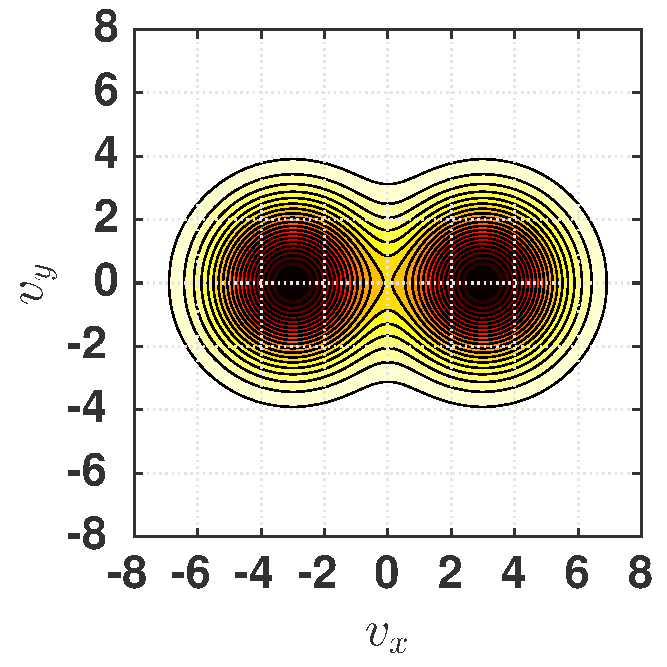
\includegraphics[width=0.95\columnwidth]{full_001.pdf}}
    \end{column}
  \end{columns}
\end{frame}

%------------------------------------------------------------------------
\begin{frame}
  \frametitle{Nonlinear bi-Maxwellian relaxation\\
    \textcolor{egg}{\large Contours illustrating time-evolution}}
  \begin{center}
    \visible<1->{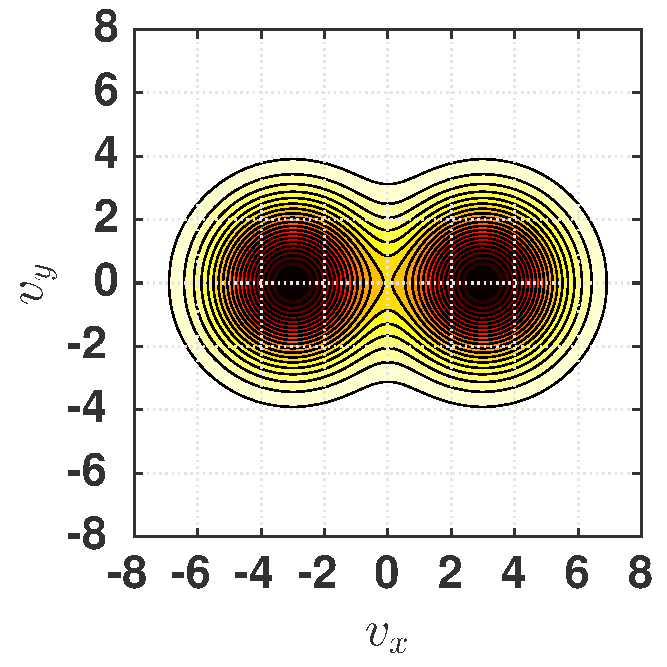
\includegraphics[width=0.32\textwidth]{full_001.pdf}}
    \visible<2->{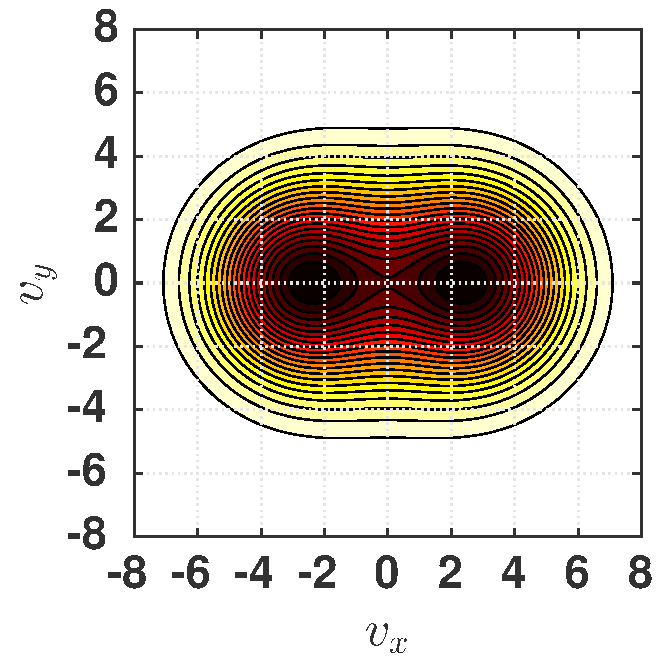
\includegraphics[width=0.32\textwidth]{full_002.pdf}}
    \visible<3->{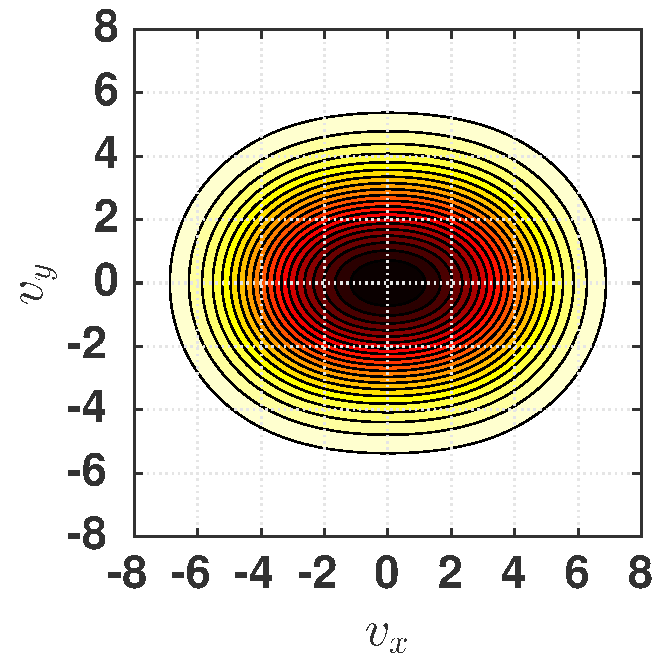
\includegraphics[width=0.32\textwidth]{full_003.pdf}}
  \end{center}
\end{frame}
  
%------------------------------------------------------------------------
\begin{frame}
  \frametitle{Nonlinear bi-Maxwellian relaxation\\
    \textcolor{egg}{\large Contours illustrating time-evolution}}
  \begin{center}
    {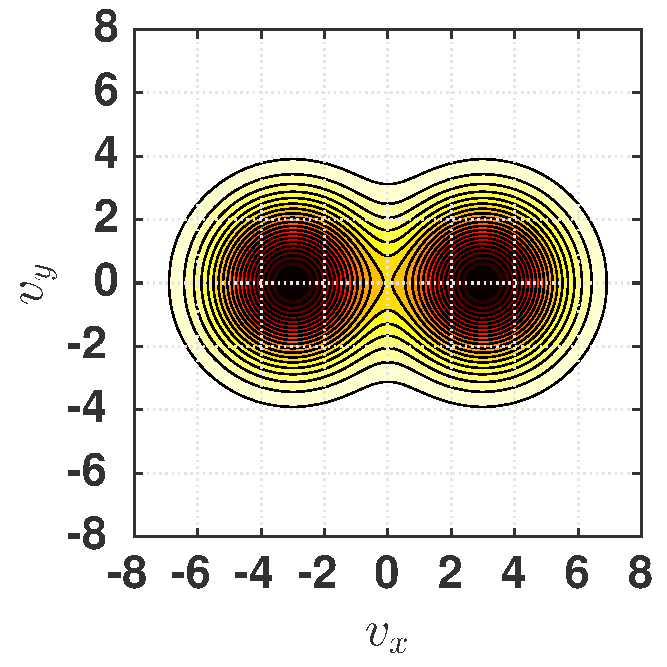
\includegraphics[width=0.4\textwidth]{full_001.pdf}}
    {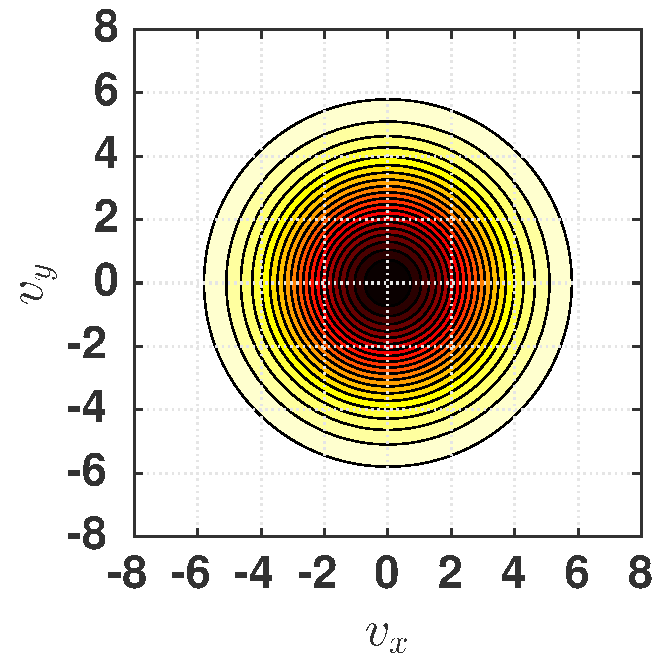
\includegraphics[width=0.4\textwidth]{full_004.pdf}}
  \end{center}
\end{frame}
  
%-----------------------------------------------------------------------
\begin{frame}
  \frametitle{Nonlinear bi-Maxwellian relaxation\\
    \textcolor{egg}{\large 3D versus 2D}}
  $\hilite{3D}\quad F_s^i(\mathbf{v})=\left(\gamma_s^i/\pi\right)^{3/2}
  \exp{[-\gamma_s^i(\mathbf{v}-\mathbf{v}_s^i)^2]}$
\vspace{-1mm}
  \begin{center}
  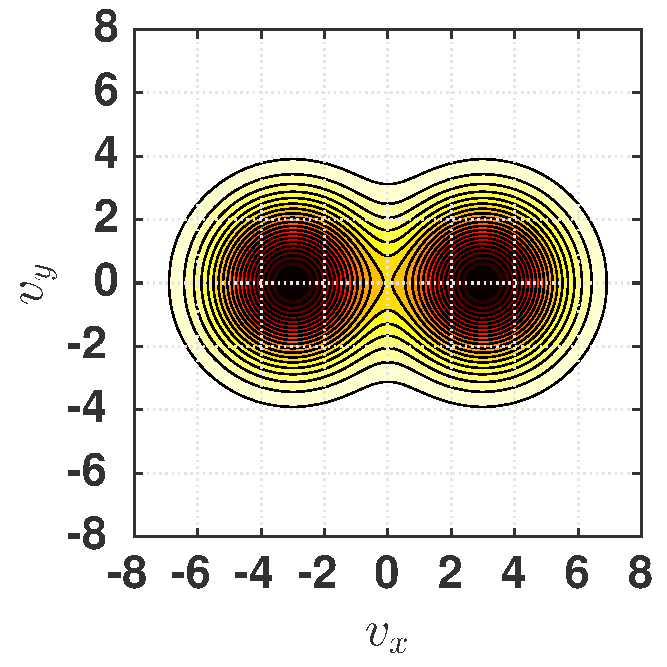
\includegraphics[width=0.22\textwidth]{full_001.pdf}
  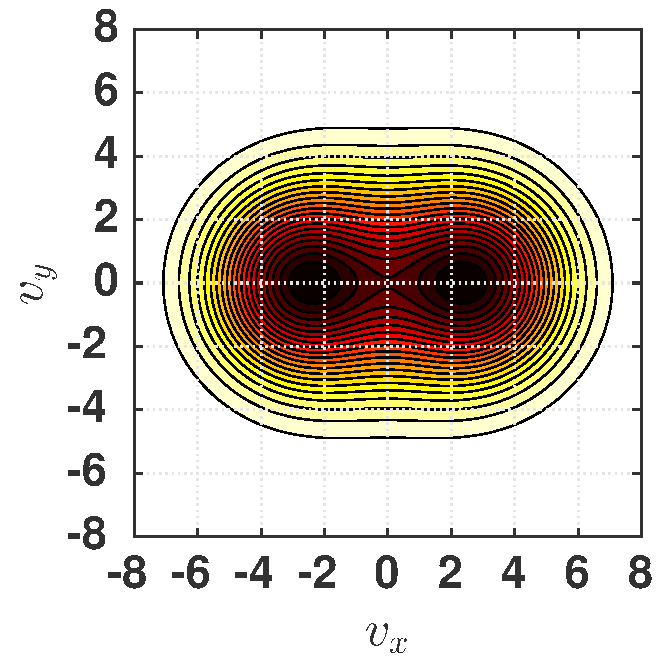
\includegraphics[width=0.22\textwidth]{full_002.pdf}
  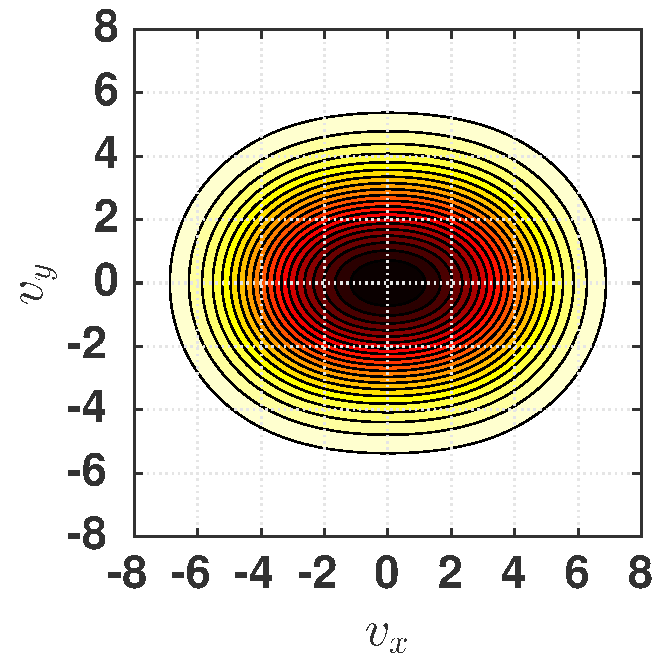
\includegraphics[width=0.22\textwidth]{full_003.pdf}
  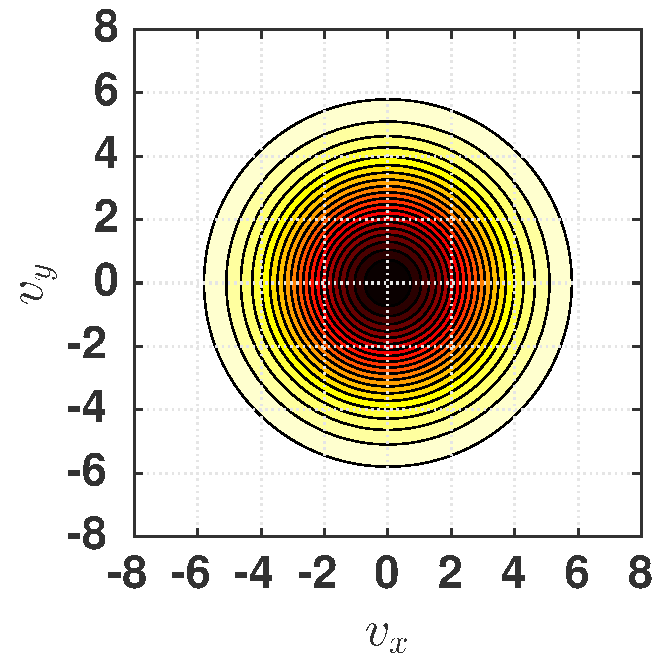
\includegraphics[width=0.22\textwidth]{full_004.pdf}
\end{center}
\vskip -2mm
$\hilite{2D}\quad F_s^i(\mathbf{v})=(\gamma_s^i/\pi)^{3/2}
I_0(2\gamma_s^iv_{s,\perp}^iv_{\perp})
e^{-\gamma_s^i(v_{\parallel}-v_{s,\parallel}^i)^2-\gamma_s^i(v_{\perp}^2+(v_{s,\perp}^i)^2)}$
\vspace{-1mm}
\begin{center}
  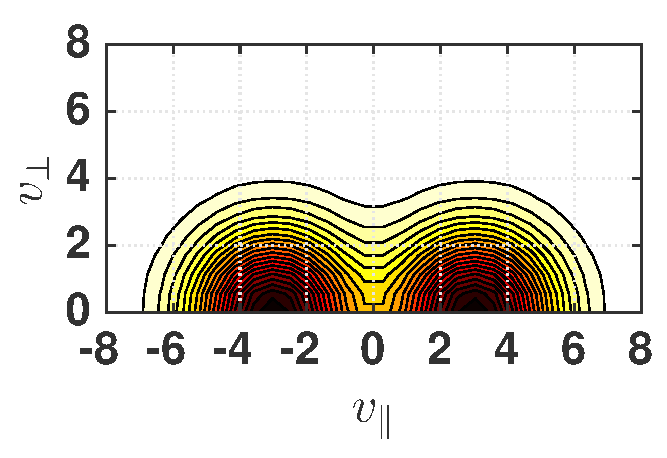
\includegraphics[width=0.22\textwidth]{axisymmetric_001.pdf}
  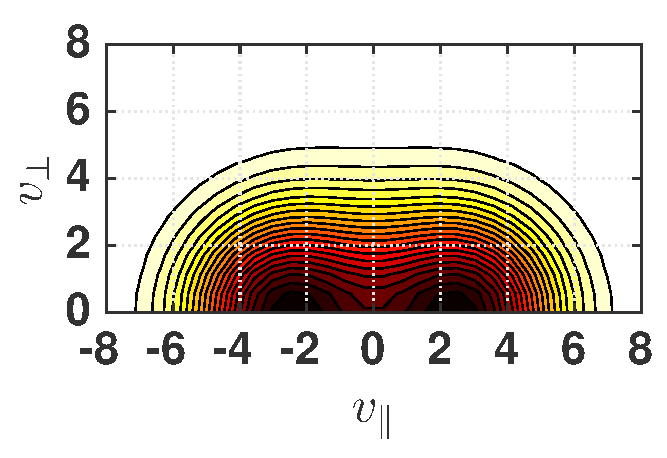
\includegraphics[width=0.22\textwidth]{axisymmetric_002.pdf}
  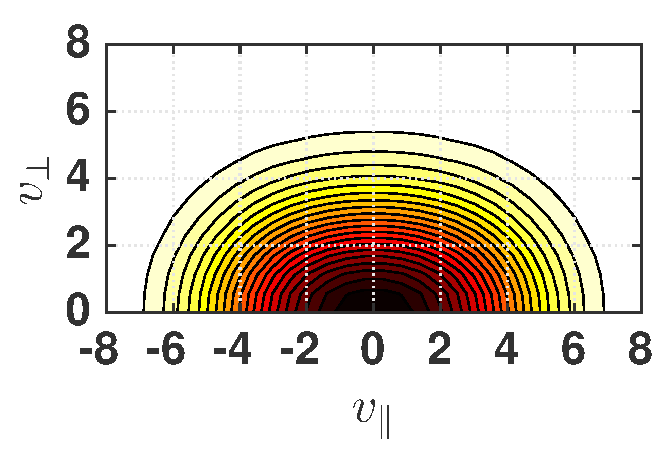
\includegraphics[width=0.22\textwidth]{axisymmetric_003.pdf}
  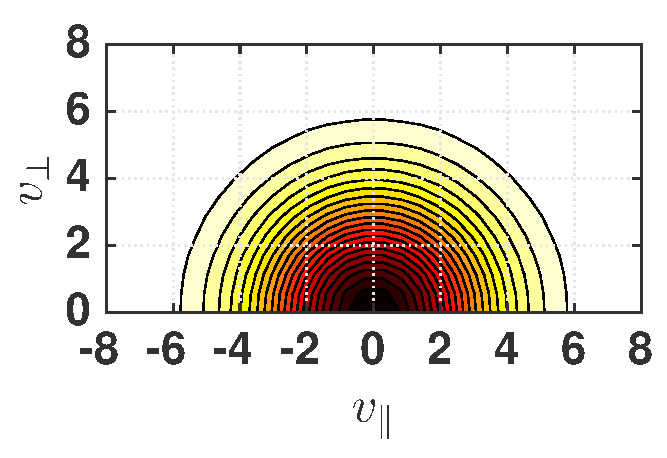
\includegraphics[width=0.22\textwidth]{axisymmetric_004.pdf}
\end{center}
\end{frame}
%-----------------------------------------------------------------------------
